%
% teil1.tex -- Beispiel-File für das Paper
%
% (c) 2020 Prof Dr Andreas Müller, Hochschule Rapperswil
%
% !TEX root = ../../buch.tex
% !TEX encoding = UTF-8
%
\section{Allgemeiner Aufbau einer Mödius Transformation
\label{moebius:section:teil1}}
\kopfrechts{Allgemeiner Aufbau einer Mödius Transformation}

Eine Möbius Transformation kann man als Kombinationen von einfachen Transformationen verstehen.
Es gibt drei Arten von diesen Transformationen.

\textbf{Die Translation:}

\[
z \mapsto z + b
\]

Sie verschiebt jeden Punkt der komplexen Ebene um die komplexe Zahl b

\begin{figure}[h]
	\centering
	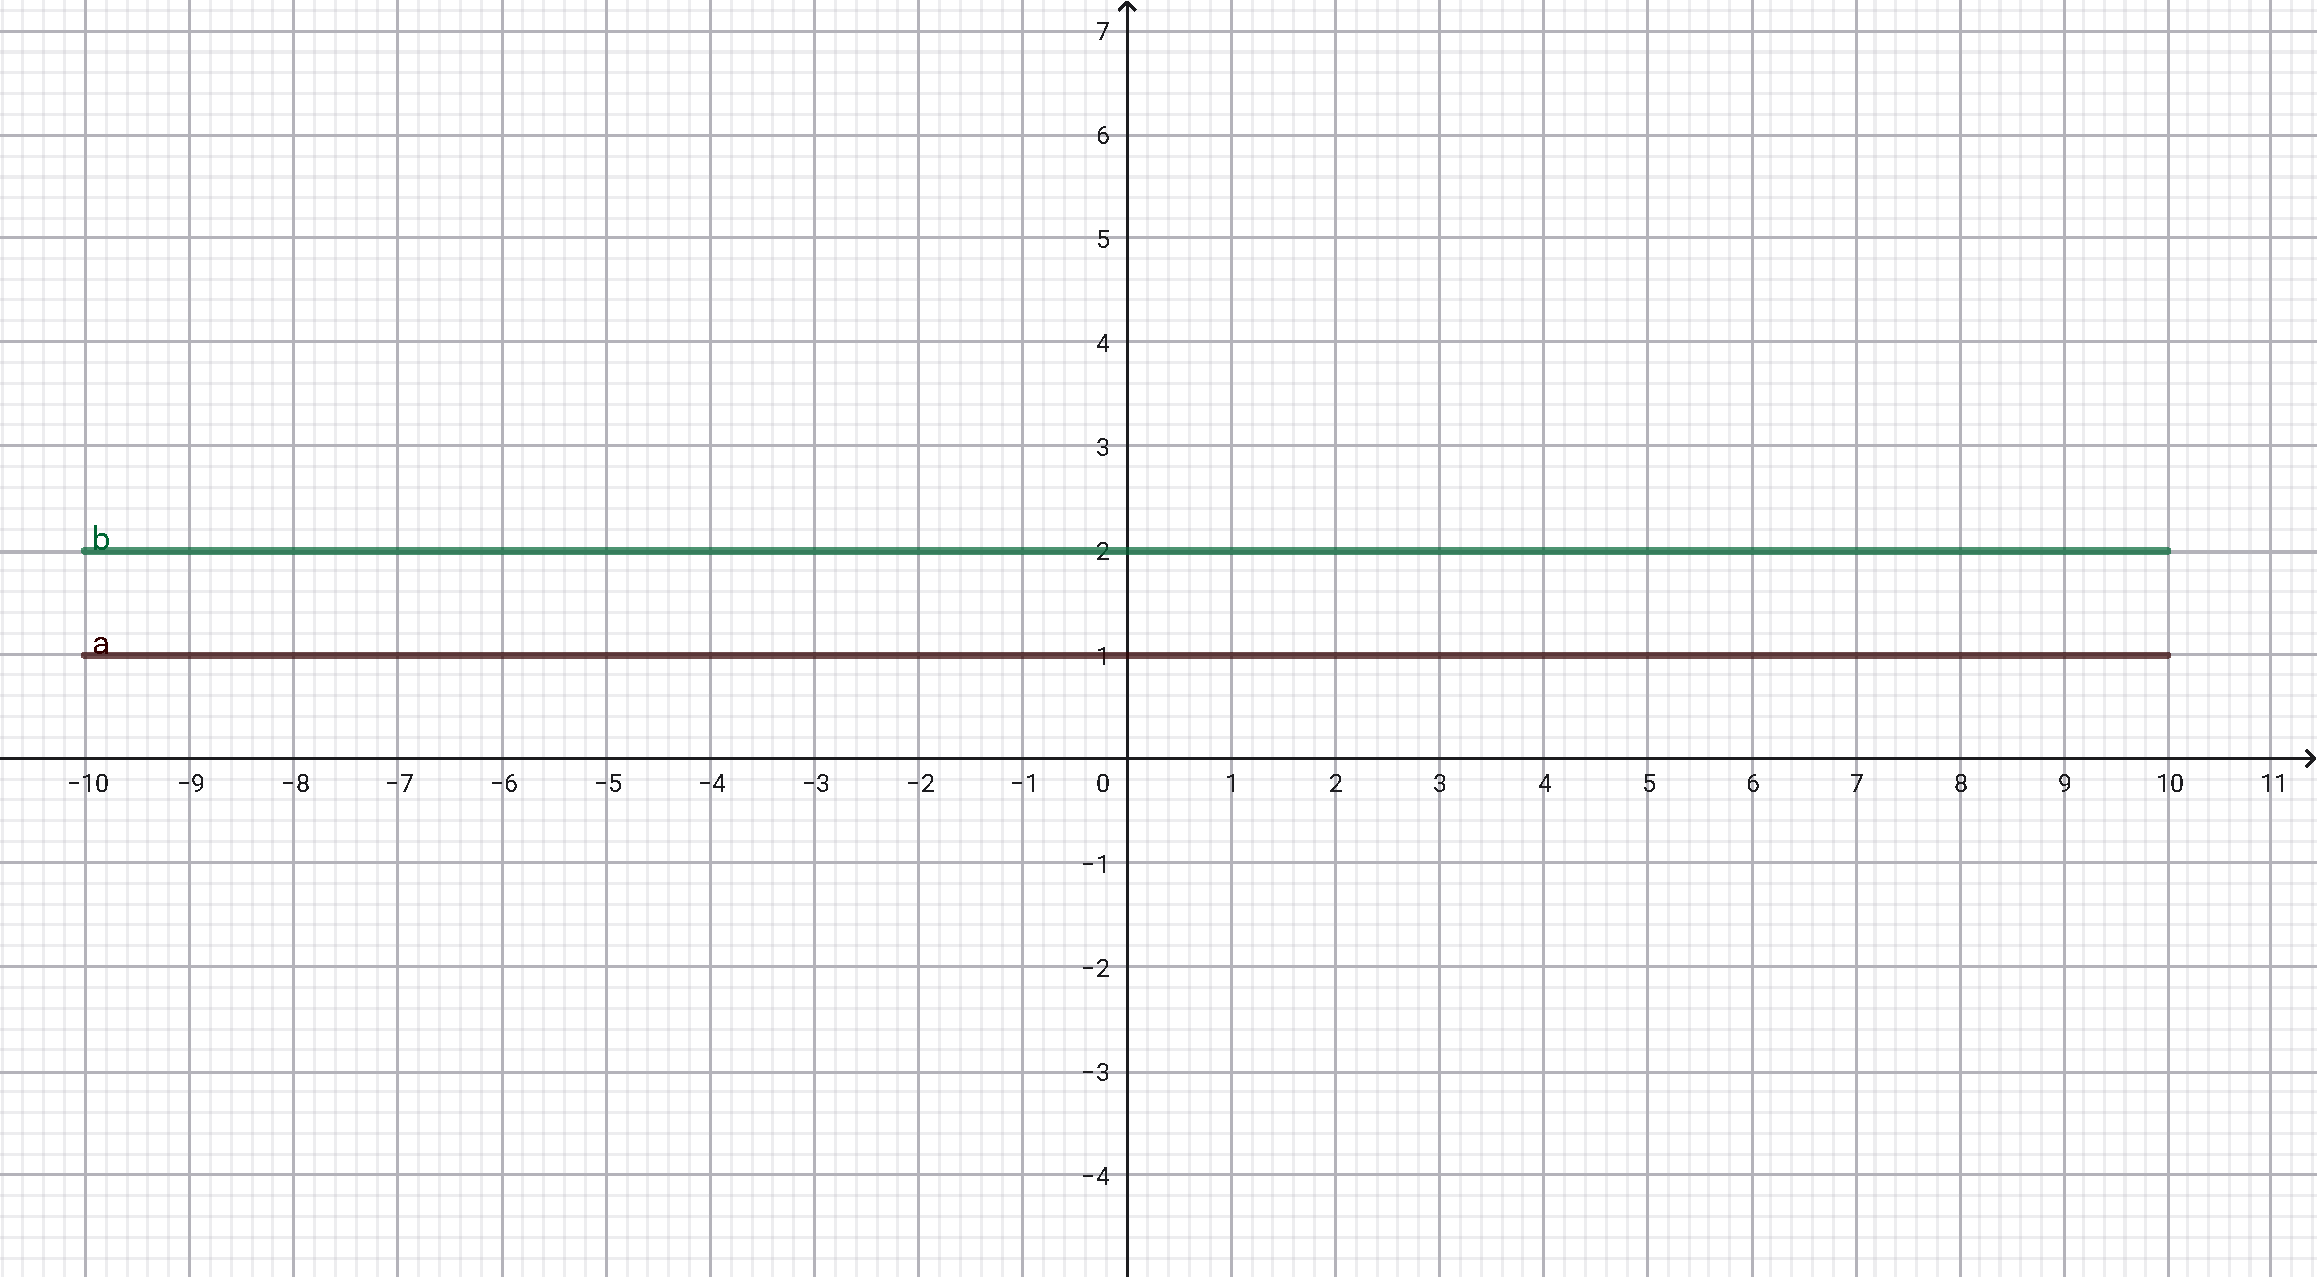
\includegraphics[width=0.6\textwidth]{bild5.pdf}
	\caption{Verschiebung des Imaginärteils}
\end{figure}


\textbf{Die Skalierung und Rotation:}

\[
z \mapsto az
\]

Diese Transformation beschreibt eine Streckung und gleichzeitig eine Rotation der komplexen Ebene um den Ursprung.

\begin{figure}[h]
	\centering
	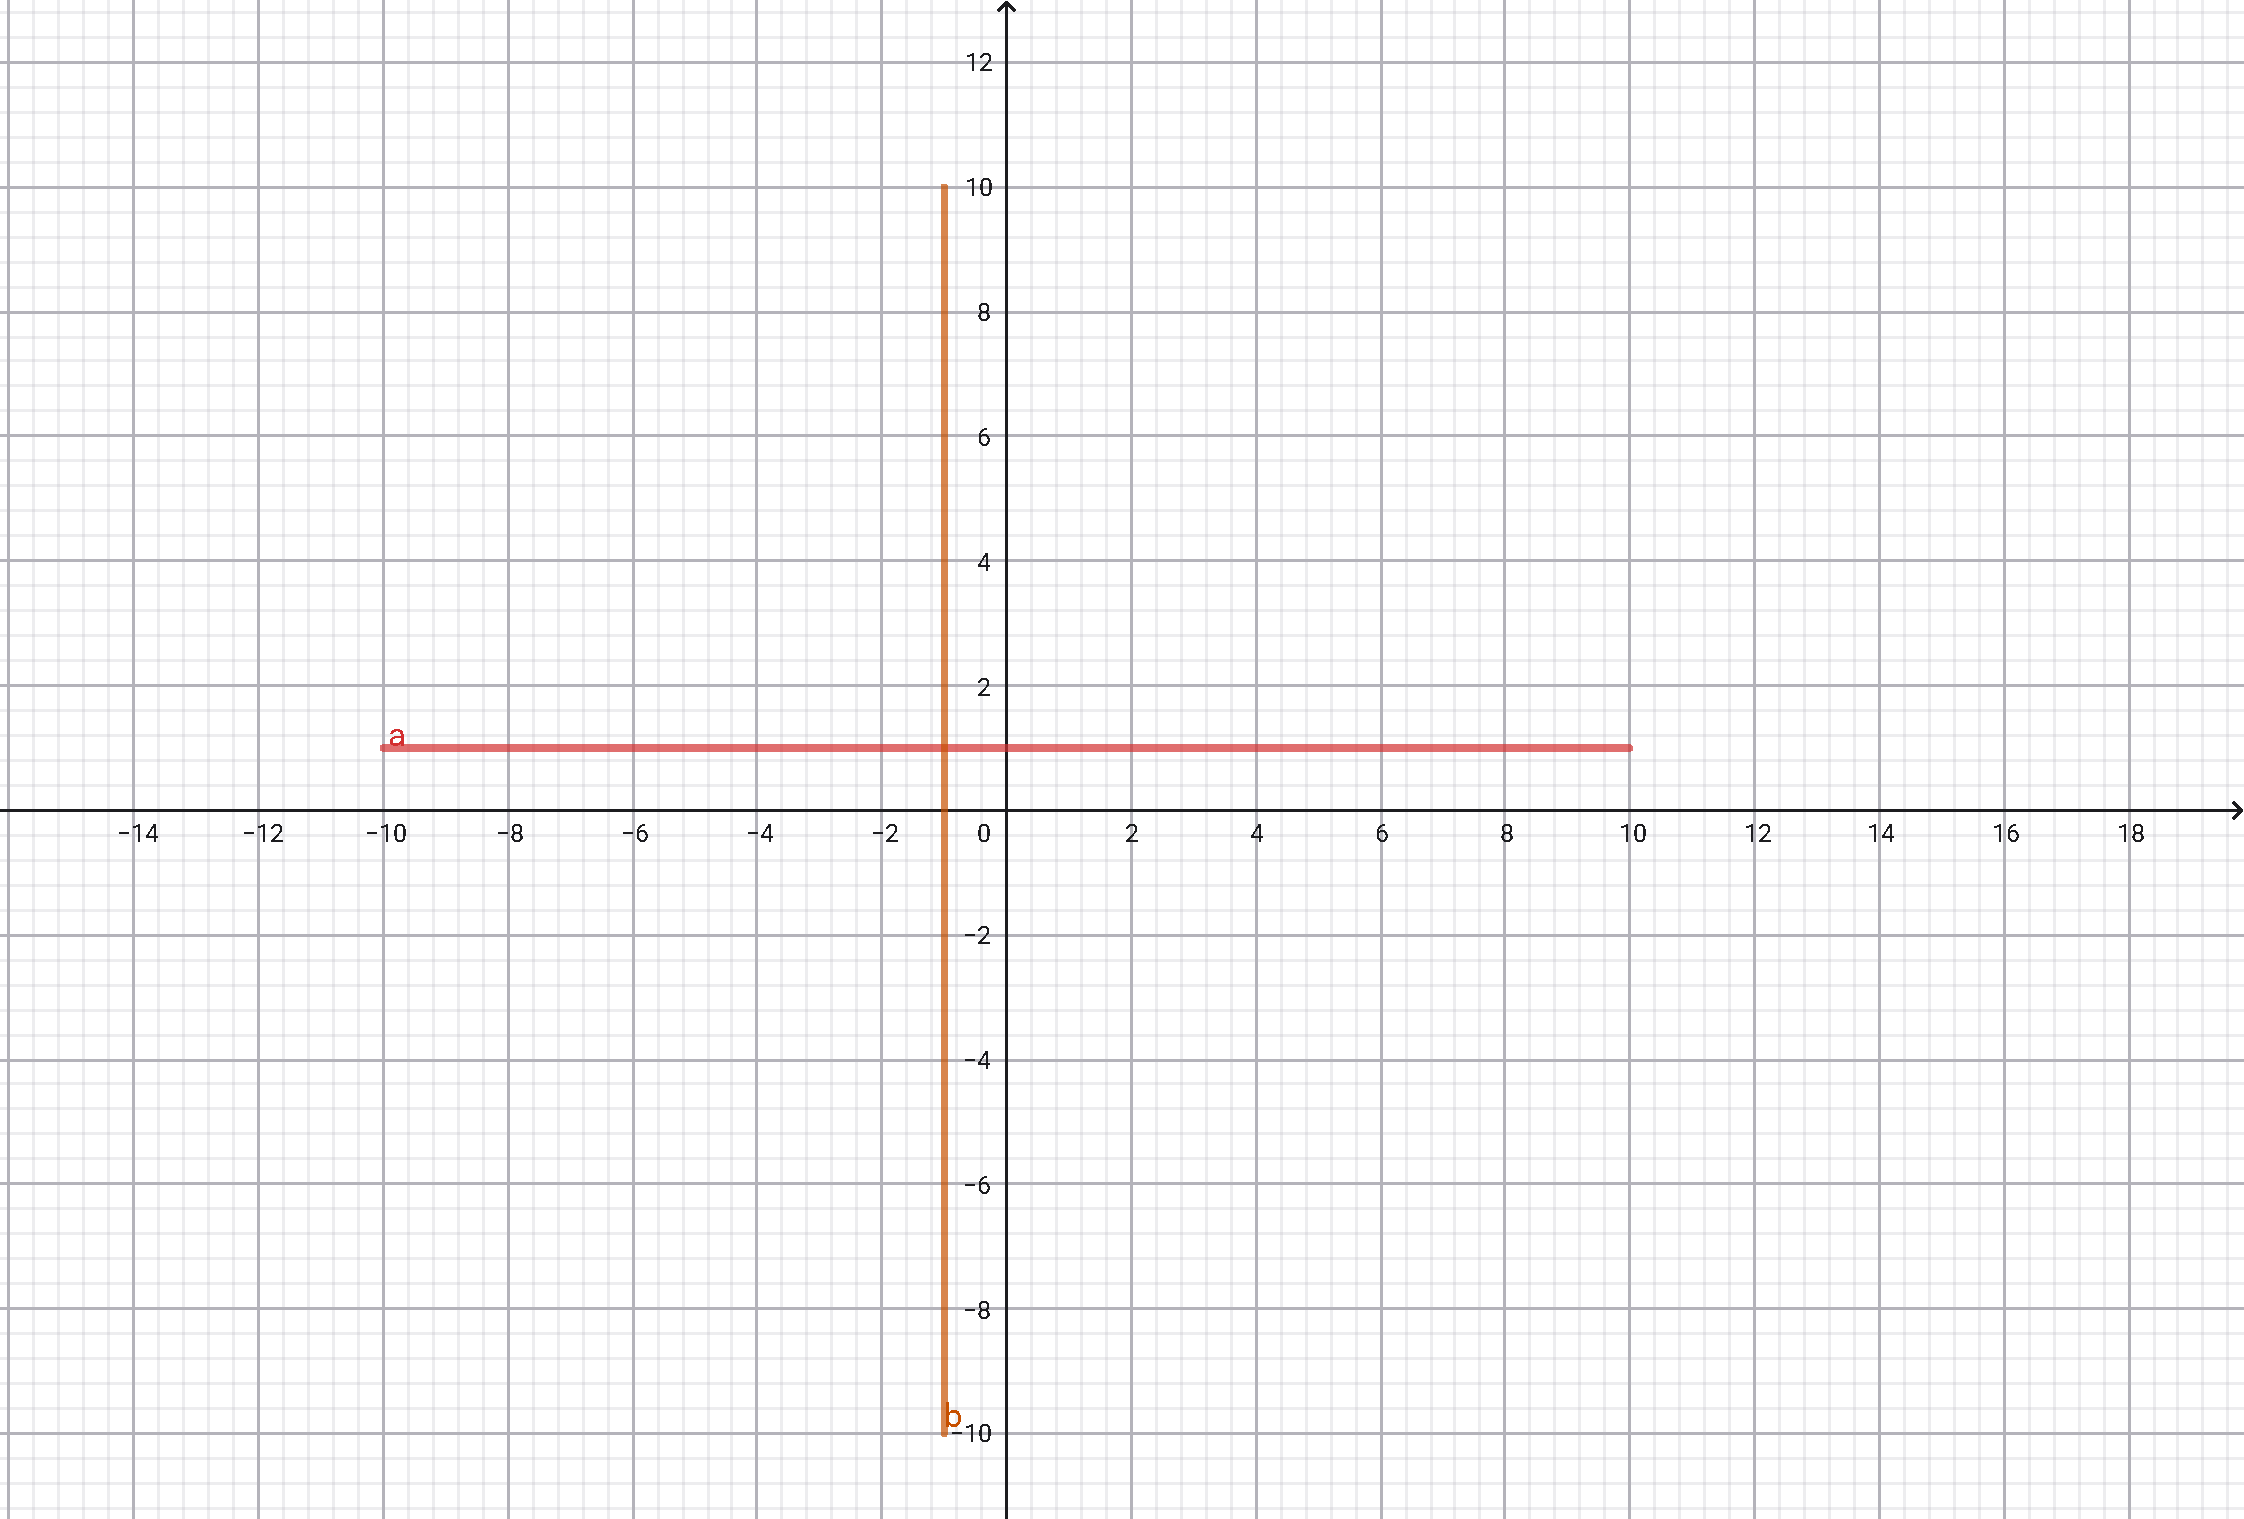
\includegraphics[width=0.6\textwidth]{bild3.pdf}
	\caption{Drehung um 90 Grad}
\end{figure}

Für die Rotation wird für $a = e^{i\varphi}$ eingesetzt.


\textbf{Die Inversion:}

\[
z \mapsto \frac{1}{z}
\]

Die Inversion bildet jeden Punkt der komplexen Ebene auf seinen Kehrwert ab und ist verantwortlich für die charakteristische Abbildung von Geraden auf Kreise und umgekehrt.

\begin{figure}[h]
	\centering
	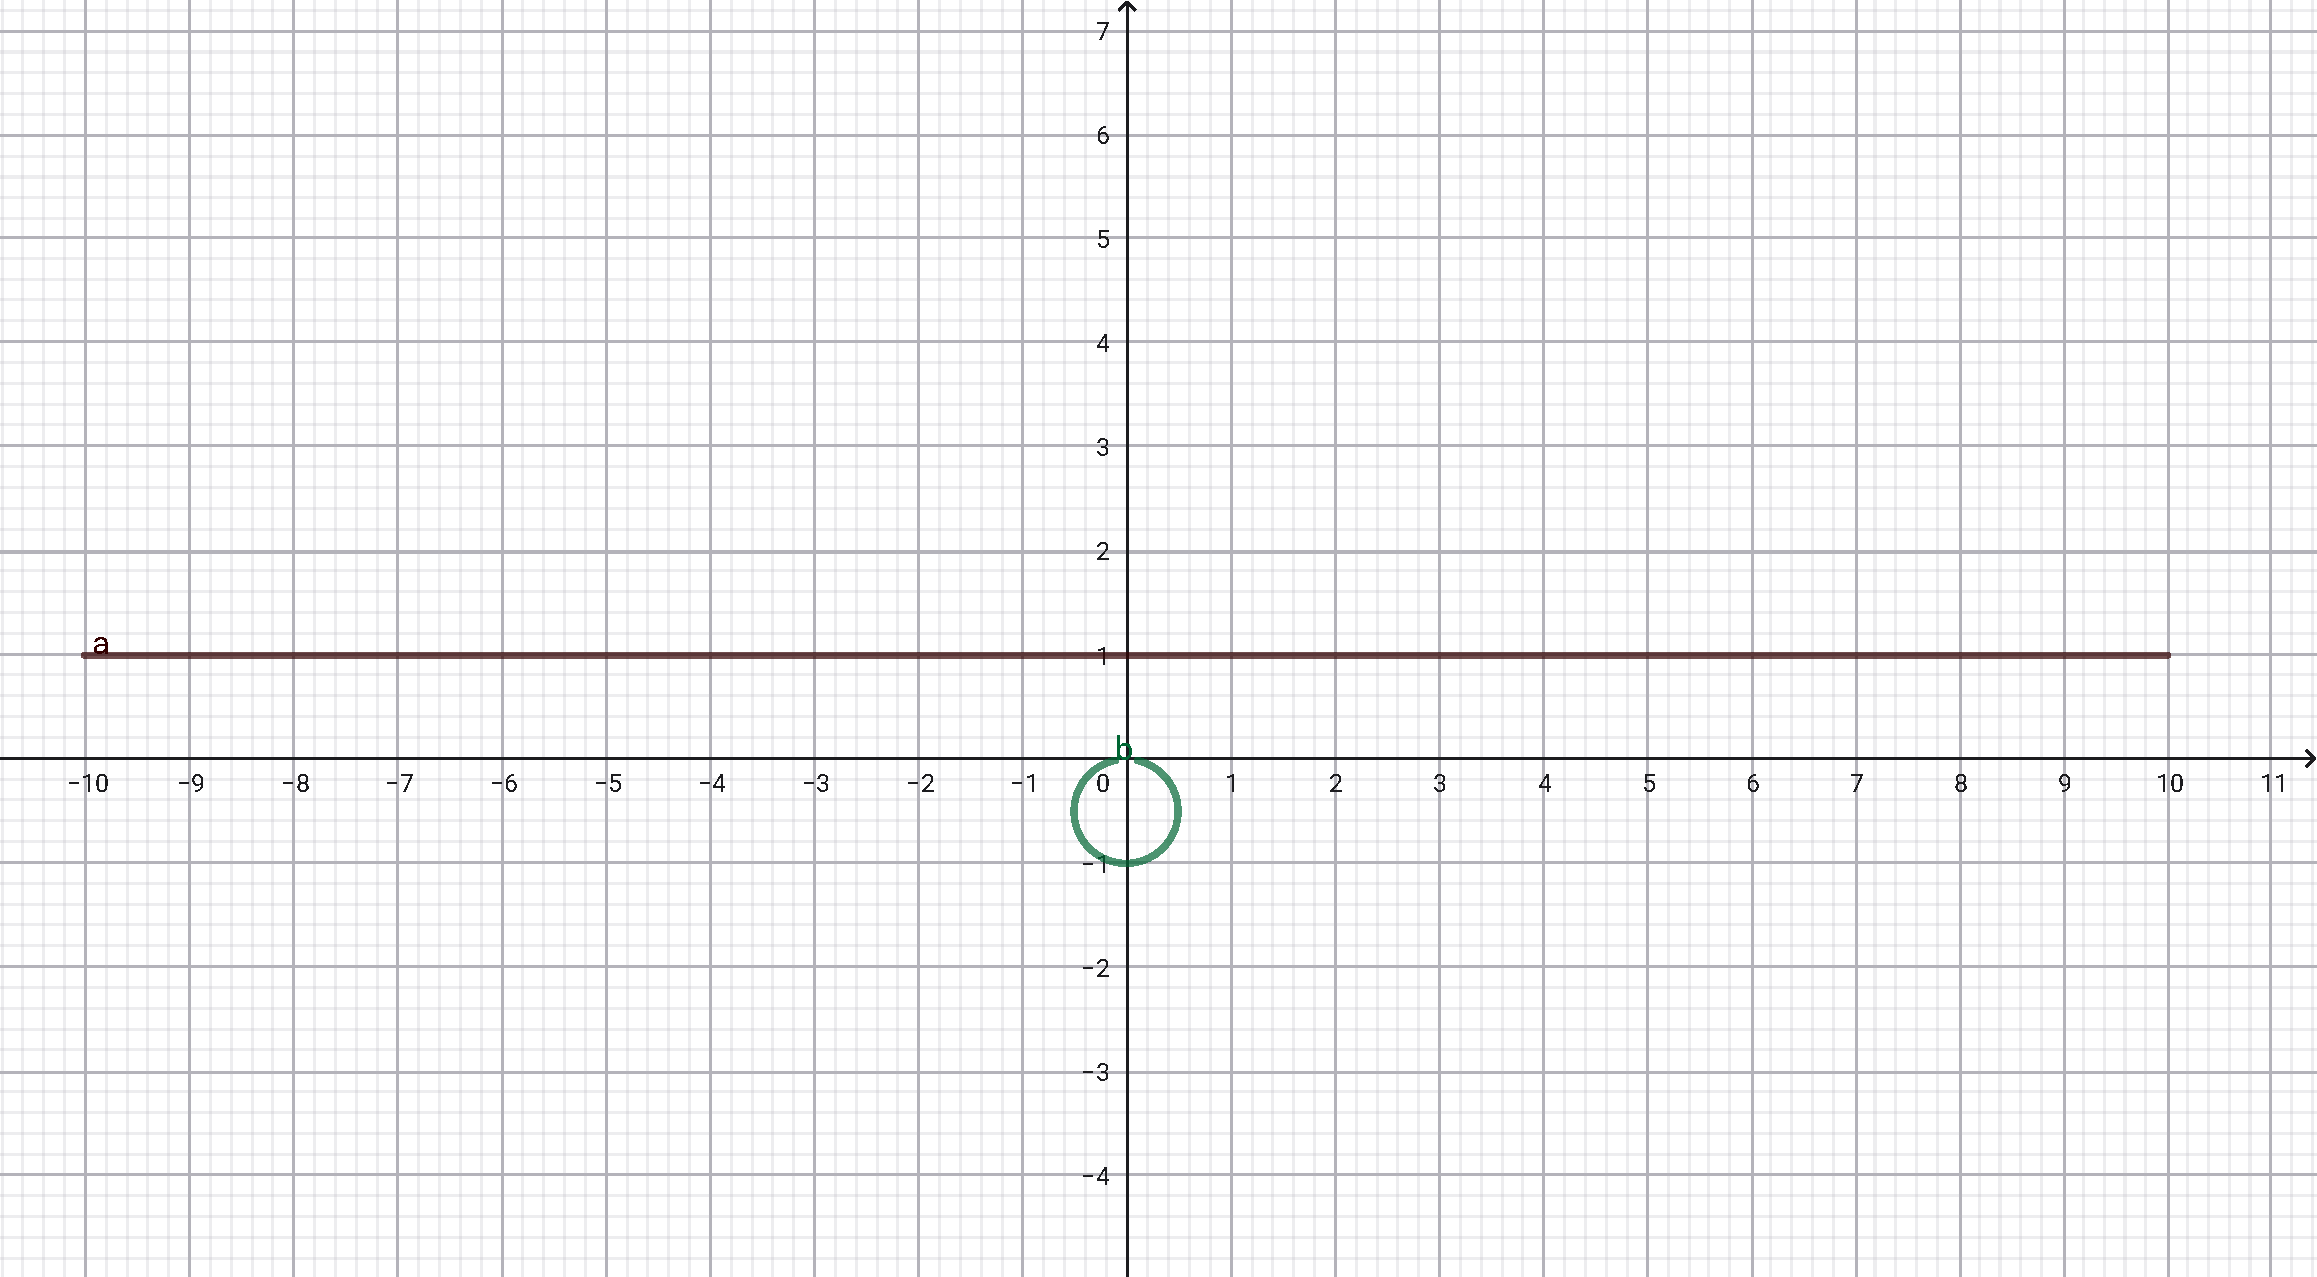
\includegraphics[width=0.6\textwidth]{bild4.pdf}
	\caption{Gerade zu Kreis}
\end{figure}


\textbf{Die Allgemeine Form einer Möbius Transformation:}

\[
f(z) = \frac{a z + b}{c z + d}, \quad a,b,c,d \in \mathbb{C}, \; ad - bc \neq 0
\]

kann als Verkettung von Translation, Skalierung/Rotation und Inversion verstanden werden.

\[ad - bc \neq 0\]

Dies ist notwendig, da die Transformation sonst degeneriert. Für \(ad - bc = 0\) wäre die Abbildung nicht mehr invertierbar und würde die gesamte Ebene auf eine konstante oder eindimensionale Menge abbilden.

Möbius-Transformationen sind bijektiv.

Das bedeutet, dass sie sowohl injektiv als auch surjektiv sind:

\begin{itemize}
	\item \textbf{Injektiv:} Verschiedene Punkte der Definitionsmenge werden auf verschiedene Punkte abgebildet.
	\item \textbf{Surjektiv:} Jeder Punkt der Zielmenge wird von mindestens einem Punkt der Definitionsmenge getroffen.
\end{itemize}

Damit ist jede Möbius-Transformation umkehrbar, d.\,h. es existiert eine inverse Möbius-Transformation.
